% Horizon production RL loop: system-level pipeline diagram
% Chapter 13: Reinforcement Learning in the Field
% Standalone TikZ diagram -- compile with: pdflatex horizon_pipeline.tex
% Anchored to Gauci et al. (2019), arXiv 1811.00260, sections 2, 4, 5, 6, 7, 8, 9.1.

\documentclass[tikz,border=8pt]{standalone}
\usepackage{amsmath,amssymb}
\usetikzlibrary{arrows.meta, positioning, calc, fit, backgrounds}

% Project palette (from docs/compile_chapter.tex)
\definecolor{rlblue}{HTML}{4878A8}
\definecolor{rlorange}{HTML}{D4915C}
\definecolor{rlgreen}{HTML}{6BA368}
\definecolor{rlred}{HTML}{C25B56}
\definecolor{rlpurple}{HTML}{8B7BAF}
\definecolor{rlgray}{HTML}{888888}
\definecolor{rlblack}{HTML}{2D2D2D}

\begin{document}
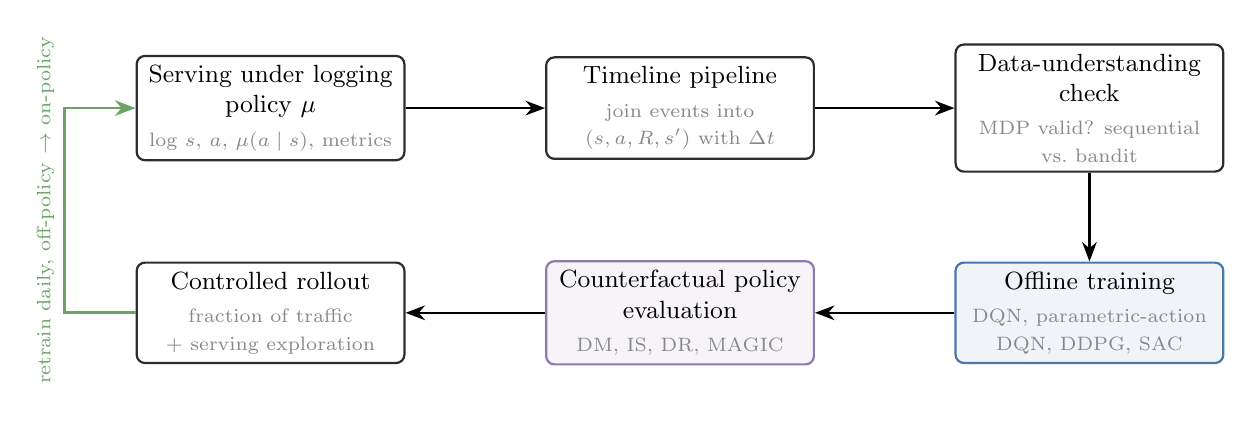
\begin{tikzpicture}[
    >=Stealth,
    stage/.style={
        draw=rlblack, rounded corners=3pt, minimum width=3.4cm,
        minimum height=1.25cm, align=center, font=\small,
        fill=white, line width=0.8pt
    },
    learn/.style={ stage, draw=rlblue, fill=rlblue!8 },
    eval/.style={ stage, draw=rlpurple, fill=rlpurple!8 },
    every edge/.style={draw, ->, >=Stealth, line width=0.9pt},
    sub/.style={font=\scriptsize, color=rlgray},
]

% ---- top row, left to right ----
\node[stage] (serve)  at (0, 2.6)
    {Serving under logging\\ policy $\mu$\\[1pt]{\scriptsize\color{rlgray} log $s,\,a,\,\mu(a\mid s)$, metrics}};
\node[stage] (timeline) at (5.2, 2.6)
    {Timeline pipeline\\[1pt]{\scriptsize\color{rlgray} join events into}\\[-1pt]{\scriptsize\color{rlgray} $(s,a,R,s')$ with $\Delta t$}};
\node[stage] (check) at (10.4, 2.6)
    {Data-understanding\\ check\\[1pt]{\scriptsize\color{rlgray} MDP valid? sequential}\\[-1pt]{\scriptsize\color{rlgray} vs.\ bandit}};

% ---- bottom row, right to left ----
\node[learn] (train) at (10.4, 0)
    {Offline training\\[1pt]{\scriptsize\color{rlgray} DQN, parametric-action}\\[-1pt]{\scriptsize\color{rlgray} DQN, DDPG, SAC}};
\node[eval] (cpe) at (5.2, 0)
    {Counterfactual policy\\ evaluation\\[1pt]{\scriptsize\color{rlgray} DM, IS, DR, MAGIC}};
\node[stage] (rollout) at (0, 0)
    {Controlled rollout\\[1pt]{\scriptsize\color{rlgray} fraction of traffic}\\[-1pt]{\scriptsize\color{rlgray} $+$ serving exploration}};

% ---- forward edges ----
\draw (serve) edge (timeline);
\draw (timeline) edge (check);
\draw (check) edge (train);
\draw (train) edge (cpe);
\draw (cpe) edge (rollout);

% ---- feedback edge: rollout back up to serving (close the loop) ----
\draw[->, >=Stealth, line width=1.0pt, rlgreen]
    (rollout.west) -- ++(-0.9,0) |- (serve.west)
    node[pos=0.25, sub, text=rlgreen, rotate=90, anchor=south]
        {retrain daily, off-policy $\to$ on-policy};

\end{tikzpicture}
\end{document}
